\intermediate{\subsection{Downloads and Installations}}

\step{Download and install \beast.}{
    \beast is available at
    \href{http://beast.bio.ed.ac.uk/Main_Page}{\url{http://beast.bio.ed.ac.uk/Main_Page}}.
    This tutorial is written for version 1.7.5 of \beast.
}

\step{Download the data and other files from Google Drive.}{
    Download the \localfile{div-time-tutorial.zip} archive from
    \href{http://www.phyletica.com/downloads/div-time-tutorial.zip}{\url{http://www.phyletica.com/downloads/div-time-tutorial.zip}}
    to your desktop, and unzip the archive.
    You should now have a \localfile{div-time-tutorial} folder on your desktop,
    and it should contain the files and folders shown in
    Box~\ref{box:tutorialDir}.

    \begin{textbox}
        \centering
        \fbox{\begin{minipage}[c][10em][c]{0.5\textwidth}
            \ttfamily
            \begin{compactitem}
                \item div-time-tutorial/
                \begin{compactitem}
                    \item crocodylia-cytb.nex
                    \item yule.py
                    \item output/
                    \begin{compactitem}
                        \item crocodylia-cytb-run1.log
                        \item crocodylia-cytb-run2.log
                        \item crocodylia-cytb-run1.trees
                        \item crocodylia-cytb-run2.trees
                    \end{compactitem}
                \end{compactitem}
            \end{compactitem}
        \end{minipage}}
        \caption{The files required for this tutorial.}
        \label{box:tutorialDir}
    \end{textbox}
}

\intermediate{\subsection{Setting up XML file with \program{BEAUTi}}}

\step{Launch BEAUTi.}{Begin by launching the \program{BEAUTi} program. If you
    are using Mac OSX or Windows, you should be able to do this by double
    clicking on the application. If everything is working correctly, a window
    should appear that looks something like Figure~\ref{fig:beautiInit}.
    \begin{figure}[htbp]
        \centering
        \fbox{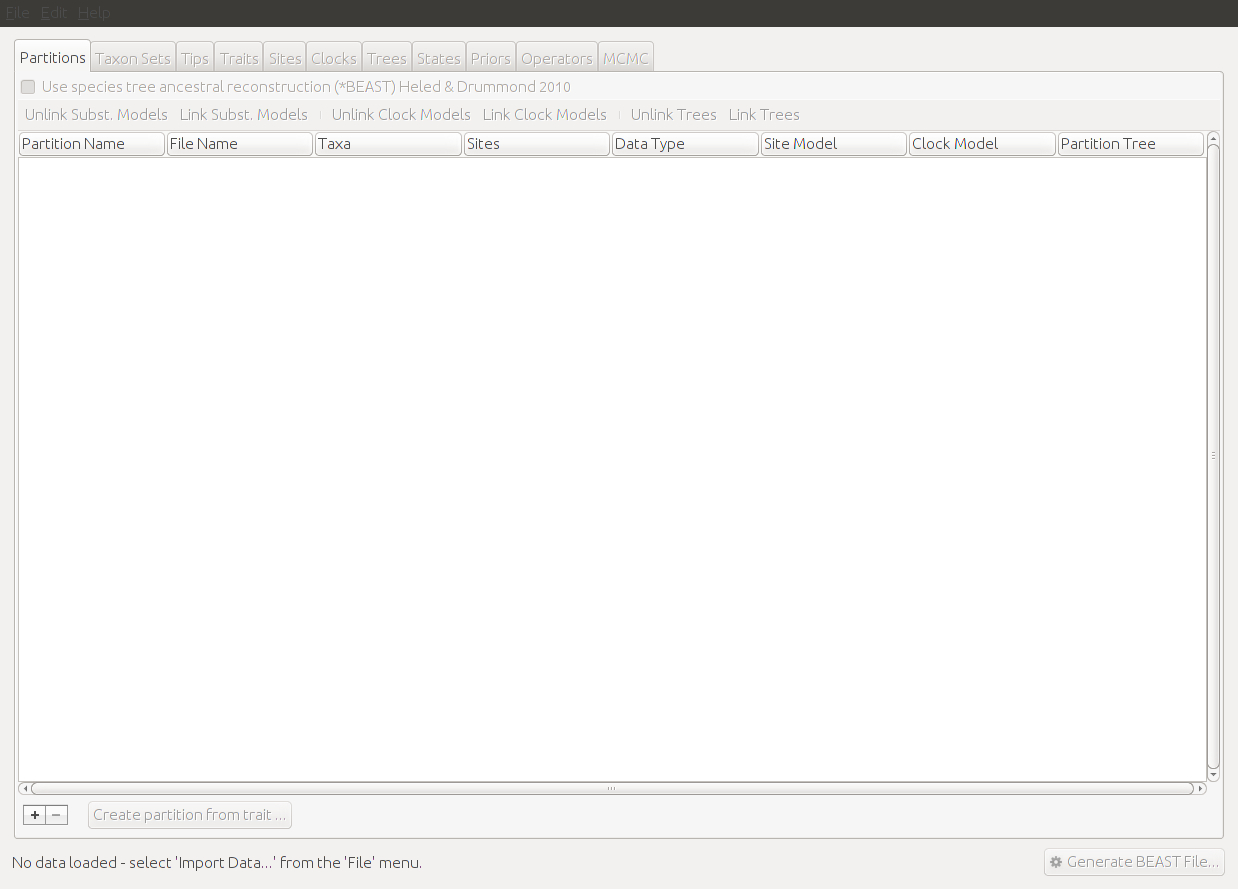
\includegraphics[width=0.7\textwidth]{../screenshots/beauti-init.jpg}}
        \caption{BEAUTi window.}
        \label{fig:beautiInit}
    \end{figure}
}

\step{Import the data in \localfile{crocodylia-cytb.nex}.}{
    Import the sequence data from the file \localfile{crocodylia-cytb.nex}
    using the drop-down menu \subItem{File}{Import Data} or using the
    \plusbutton button near the bottom-left corner of the window.

    You should be able to confirm that \program{BEAUTi} successfully imported
    24 sequences of nucleotides of length 1137
    (Figure~\ref{fig:beautiDataImported}).
    \begin{figure}[htbp]
        \centering
        \fbox{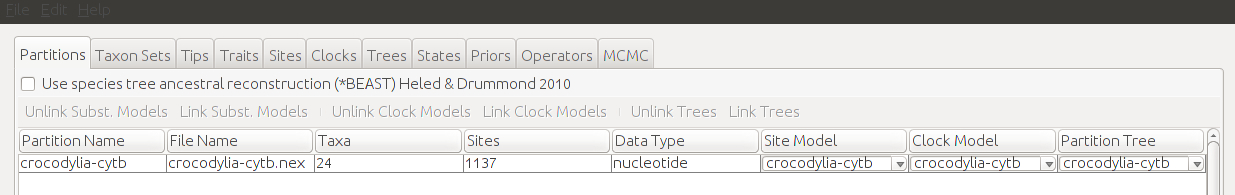
\includegraphics[width=0.8\textwidth]{../screenshots/beauti-data-imported.jpg}}
        \caption{The data successfully loaded by BEAUTi.}
        \label{fig:beautiDataImported}
    \end{figure}
}

\step{Inspect the alignment.}{
    Double click on the file name \localfile{crocodylia-cytb.nex} to bring up a
    window displaying the aligned sequences. It is always good practice to make
    sure everything looks as you expect. The cytochrome b gene is
    protein-coding, and aligns well across Crocodylia without gaps.
}

\step{Define taxon sets.}{
    Next, we need to define some sets of taxa. Later, we will be able to use
    each of these sets to place priors on the age of their most recent common
    ancestor (MRCA).
    Let's start by defining the set for the clade
    containing the fossil taxon \emph{Navajosuchus mooki}; this clade has
    the family name Alligatoridae.

    Click on the \menutab{Taxa} tab. Once in the \menutab{Taxa}
    tab, click on the \plusbutton near the bottom-left corner of the window.
    This will create an untitled taxon set in the left-most box in the window.
    Change the name of this taxon set to \taxonset{Alligatoridae} and enter \fieldvalue{65}
    into Age column. This age is simply a starting value for the age of the
    MRCA of \taxonset{Alligatoridae}. It will ensure that the initial tree used
    to start the analysis is consistent with the lower bound of our fossil
    calibration (which will be 64 million years).
    
    We do not want to constrain \taxonset{Alligatoridae} to be monophyletic, so
    leave the \field{Mono?} box unchecked. Also, we are confident that
    \emph{Navajosuchus mooki} is nested within \taxonset{Alligatoridae}, and so
    we will leave the \field{Stem?} box unchecked. Because we only have a
    single tree, you can leave the \field{Tree} column unchanged.

    Next, we need to highlight the species that belong to
    \taxonset{Alligatoridae} within the \field{Excluded Taxa} window, and move
    them over to the \field{Included Taxa} window using the ``$\to$'' button.
    \taxonset{Alligatoridae} includes the following genera:
    \begin{compactitem}
        \item \emph{Alligator}
        \item \emph{Caiman}
        \item \emph{Melanosuchus}
        \item \emph{Paleosuchus}
    \end{compactitem}
    Highlight the species for these genera and move them over to the
    \field{Included Taxa} window.
    If you did everything correctly, your BEAUTi window should look like
    Figure~\ref{fig:beautiAlligatoridae}.
    \begin{figure}[htbp]
        \centering
        \fbox{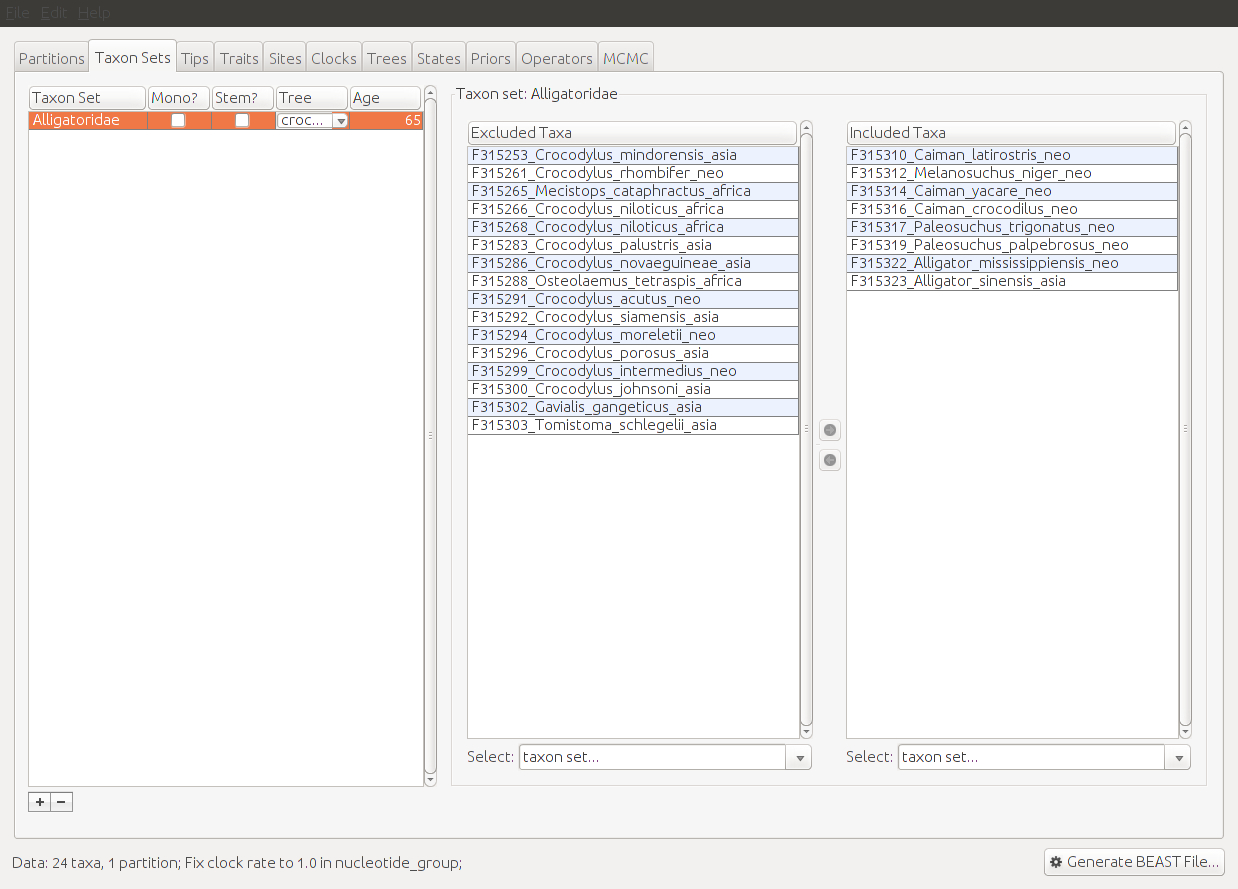
\includegraphics[width=0.9\textwidth]{../screenshots/beauti-taxon-set-alligatoridae.jpg}}
        \caption{The taxon set \taxonset{Alligatoridae} correctly defined.}
        \label{fig:beautiAlligatoridae}
    \end{figure}

    Next, let's define a taxon set for the genus \emph{Crocodylus}, which we
    will later use to specify an age prior corresponding to the fossil
    \emph{Crocodylus palaeindicus}. Click on the \plusbutton again to create a
    new taxon set, and name it \taxonset{Crocodylus}. Specify a starting age of
    \fieldvalue{13}, and leave the \field{Mono?} unchecked.

    We are confident that \emph{Crocodylus palaeindicus} is more closely
    related to all \emph{Crocodylus} species than to any other crocodylians.
    However, we are not confident that it is nested within extant species of
    \emph{Crocodylus} and suspect it is actually sister to them (as illustrated
    in Figure~\ref{fig:crocFossils}). As a result, we want to check the
    \field{Stem?} box. This specifies that the node we are interested in
    calibrating is the MRCA of all \emph{Crocodylus} sequences and their next
    closest relative (i.e., the stem node of \emph{Crocodylus}).
    Make sure the \taxonset{Crocodylus} taxon set is highlighted, and then
    highlight all the \emph{Crocodylus} species in the \field{Excluded Taxa}
    window and move them over to the \field{Included Taxa} window.

    Lastly, we need to define a taxon set for the genus \emph{Caiman}, which we
    will later use when specifying a calibration informed by the age of the
    oldest known \emph{Caiman} fossils.  Click the \plusbutton to create a new
    taxon set, name it \taxonset{Caiman}, specify a starting age of
    \fieldvalue{10}, and leave \field{Mono?} unchecked.
    As with \emph{Crocodylus} we don't know if the oldest \emph{Caiman} fossil
    taxa are nested within or sister to extant \emph{Caiman} species, and so we
    need to check the \field{Stem?} box.
    Highlight the three \emph{Caiman} species and move them over to the
    \field{Included Taxa} window.

    We will also be specifying a prior for the age of the root node of the
    tree, but we do not need to define a taxon set for this, because the root
    node is always defined by BEAUTi (you will see this later).

    Before you proceed to the next step, double check the three taxon sets
    you just defined and make sure you did not make a mistake with their
    ages or in selecting the species associated with them. Even a single
    misplaced species can lead to some very bizarre results!

    If you did everything correctly, your BEAUTi window should look similar to
    Figure~\ref{fig:beautiTaxSets}.

    \begin{figure}[htbp]
        \centering
        \fbox{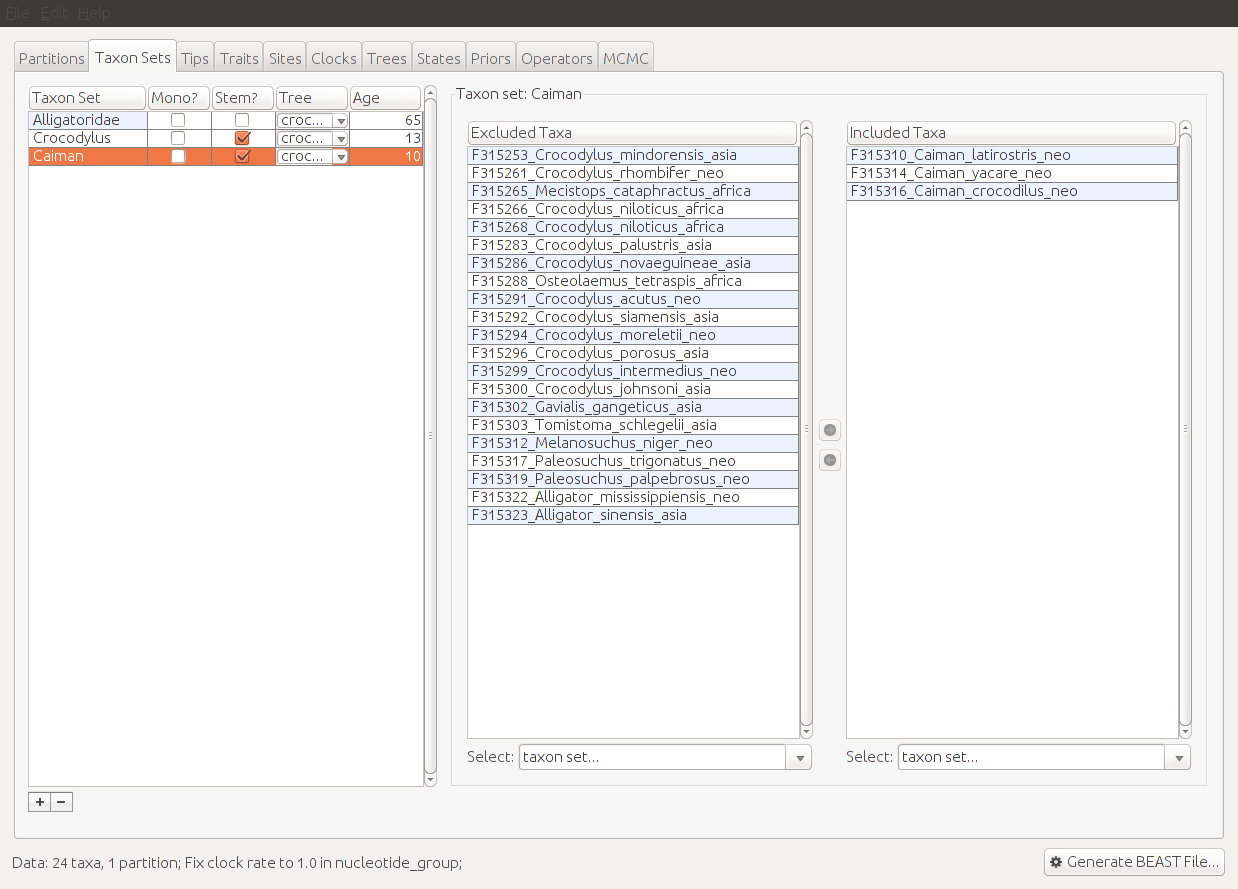
\includegraphics[width=0.9\textwidth]{../screenshots/beauti-taxon-sets.jpg}}
        \caption{All three taxon sets defined.}
        \label{fig:beautiTaxSets}
    \end{figure}
}

% \step{Define geographic traits.}{
%     Next we will use the \menutab{Traits} tab to define a new character for
%     the geographic location of each species.
%     This step is unrelated to divergence-time estimation. It will allow us to
%     estimate the geographic locations of ancestral species across the
%     phylogeny.
%     Investigators are often interested in estimating ancestral states for
%     characters of interest, so it is worth seeing how that can be done for in
%     \beast while jointly estimating the phylogeny and divergence times.
%     However, you will be learning all about ancestral character-state
%     estimation in coming weeks, and so we will gloss over a lot of details to
%     maintain the focus on divergence-time estimation.

%     Once in the \menutab{Traits} tab, click the \plusbutton button (or the
%     \field{Add trait} button). Once the \field{Create or Import Trait(s)}
%     sub-window pops up, change the \field{Name} to \fieldvalue{geography}, set
%     the \field{Type} to \fieldvalue{discrete}, and check the \field{Create a
%     corresponding data partition} box
%     (Figure~\ref{fig:beautiCreateTraitSubWindow}). Then, click \field{OK}.

%     \begin{figure}[htbp]
%         \centering
%         \fbox{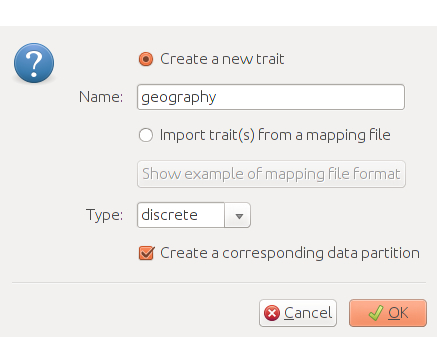
\includegraphics[width=0.4\textwidth]{../screenshots/beauti-create-trait-subwindow.jpg}}
%         \caption{Creating a new trait.}
%         \label{fig:beautiCreateTraitSubWindow}
%     \end{figure}

%     Next, click the \field{Guess trait values} button.  Once the sub-window
%     pops up, select \field{Defined by its order} and set its drop-down field to
%     \fieldvalue{last}. Put \fieldvalue{\_} (underscore) in the \field{with
%     delimiter} field (Figure~\ref{fig:beautiGuessTraitSubWindow}). Click
%     \field{OK}.
%     If successful, the \menutab{Traits} tab should look like
%     Figure~\ref{fig:beautiTraits}.

%     \begin{figure}[htbp]
%         \centering
%         \fbox{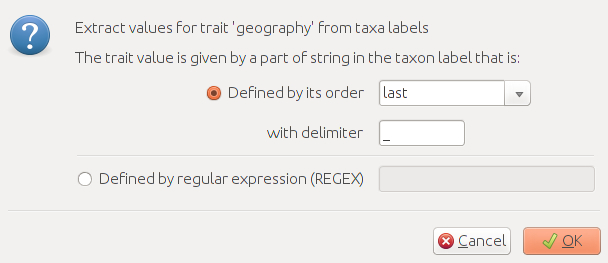
\includegraphics[width=0.5\textwidth]{../screenshots/beauti-guess-trait-subwindow.jpg}}
%         \caption{\field{Guess trait} options.}
%         \label{fig:beautiGuessTraitSubWindow}
%     \end{figure}

%     \begin{figure}[htbp]
%         \centering
%         \fbox{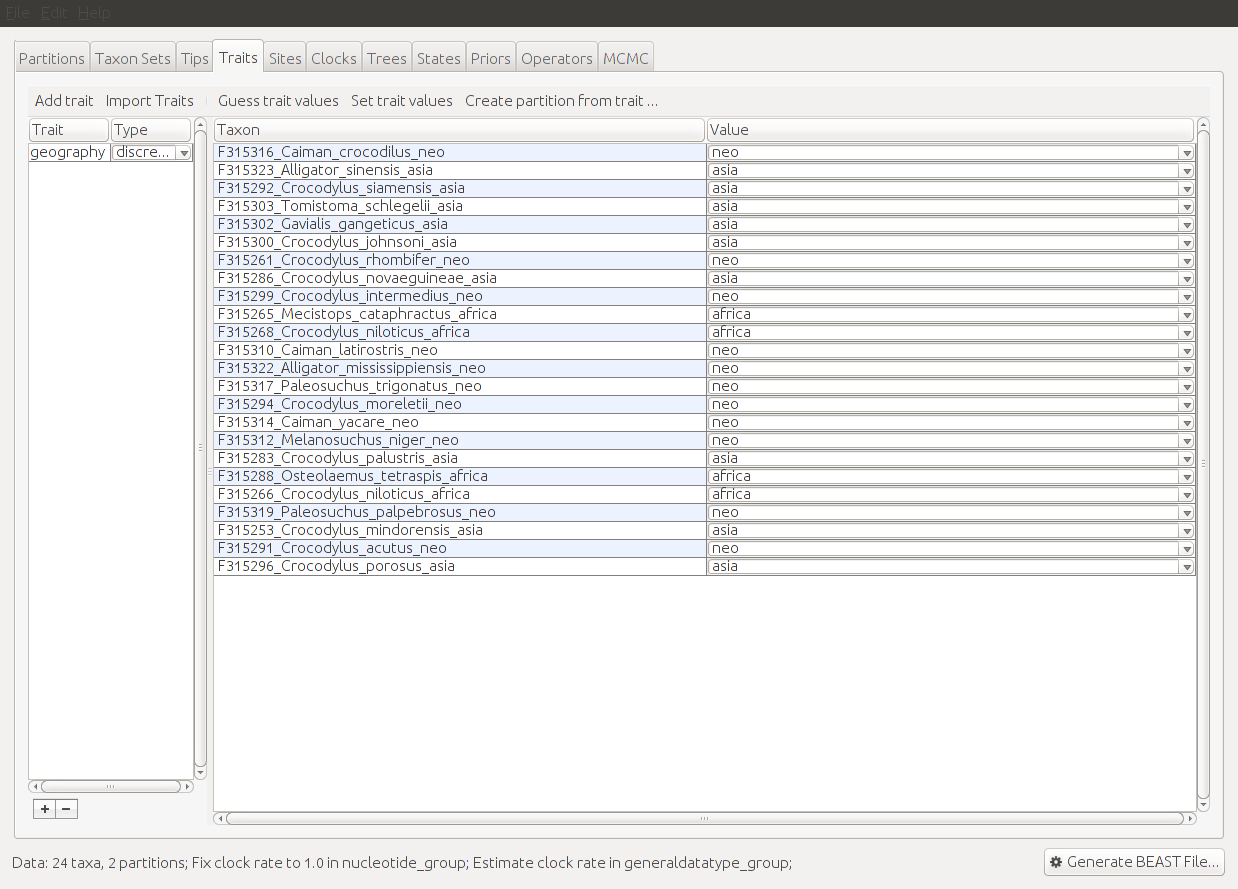
\includegraphics[width=0.8\textwidth]{../screenshots/beauti-traits.jpg}}
%         \caption{Geographic traits successfully defined.}
%         \label{fig:beautiTraits}
%     \end{figure}
% }

\step{Define Markov-chain models of substitution}{
    Next, we need to set up our continuous-time Markov chain (CTMC) model
    of nucleotide substitution under the \menutab{Sites} tab.
    Once in the \menutab{Sites} tab, and with \fieldvalue{crocodylia-cytb} selected
    in the left \field{Substitution Model} window, select the following options:
    \begin{compactdesc}
        \centering
        \item[\field{Substitution Model:}] \fieldvalue{HKY}
        \item[\field{Base frequencies:}] \fieldvalue{Estimated}
        \item[\field{Site Heterogeneity Model:}] \fieldvalue{Gamma}
        \item[\field{Number of Gamma Categories:}] \fieldvalue{4}
        \item[\field{Partition into codon positions:}] \fieldvalue{3 partitions: positions 1, 2, 3}
    \end{compactdesc}
    Lastly, check all three \field{Unlink parameters} options (Figure~\ref{fig:beautiCytbModel}).

    \begin{figure}[htbp]
        \centering
        \fbox{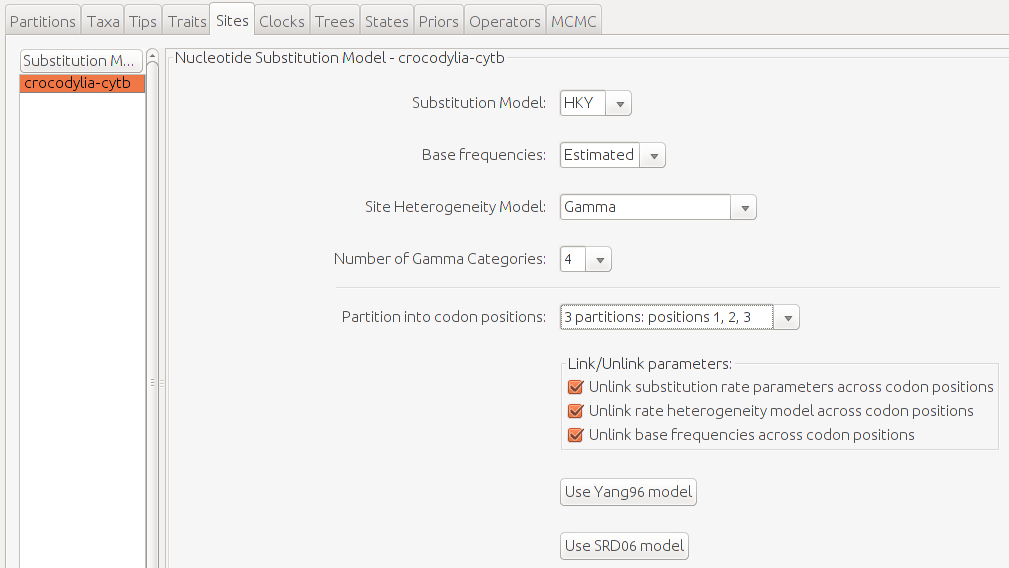
\includegraphics[width=0.8\textwidth]{../screenshots/beauti-cytb-model-no-geo.jpg}}
        \caption{The CTMC model of nucleotide substitution for cytb.}
        \label{fig:beautiCytbModel}
    \end{figure}

    % Next, select \fieldvalue{geography} in the left \field{Substitution Model}
    % window, and select \fieldvalue{Asymmetric substitution model} for the
    % \field{Discrete Trait Substitution Model} drop-down option. Check the box
    % for \field{Infer social network with BSSVS} (Figure~\ref{fig:beautiGeoModel}).

    % \begin{figure}[htbp]
    %     \centering
    %     \fbox{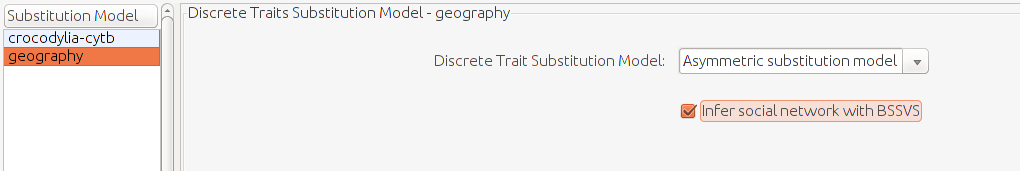
\includegraphics[width=0.8\textwidth]{../screenshots/beauti-geo-model.jpg}}
    %     \caption{The CTMC model for the geographic character.}
    %     \label{fig:beautiGeoModel}
    % \end{figure}
}

\step{Define clock models.}{
    Next, we need to move to the \menutab{Clocks} tab and specify our models of
    branch rates across the tree. BEAUTi provides one strict-clock and
    three relaxed-clock options:
    \begin{compactdesc}
        \item[\fieldvalue{Strict clock}] Assumes a constant rate of
            substitution across all the branches of the tree.
        \item[\fieldvalue{Lognormal relaxed clock (Uncorrelated)}] Assumes that
            the rates of substitution on each branch of the tree are independent
            and drawn from a single, discretized lognormal distribution
            \citep{Drummond2006}.
        \item[\fieldvalue{Exponential relaxed clock (Uncorrelated)}]  Assumes that
            the rates of substitution on each branch of the tree are independent
            and drawn from a single, exponential distribution
            \citep{Drummond2006}.
        \item[\fieldvalue{Random local clock}] Uses Bayesian stochastic search
            variable selection (BSSVS) to average over local clock models
            (i.e., it averages over the number of rate changes and their
            locations) \citep{DrummondSuchard2010}.
    \end{compactdesc}

    In general, it is best to compare (or sample over) different clock models.
    But, for the sake of keeping this tutorial simple, we will select the most
    commonly used relaxed-clock model for the cytb data.
    For the \fieldvalue{crocodylia-cytb} data, select the \fieldvalue{Lognormal
    relaxed clock (Uncorrelated)}.
    % For the \fieldvalue{geography} trait, select the \fieldvalue{Strict clock
    % model}.
    Make sure to click the \field{Estimate} box
    (Figure~\ref{fig:beautiClocks}).  You do not need to worry about the
    \field{Clock Model Group} options in the lower window.

    \begin{figure}[htbp]
        \centering
        \fbox{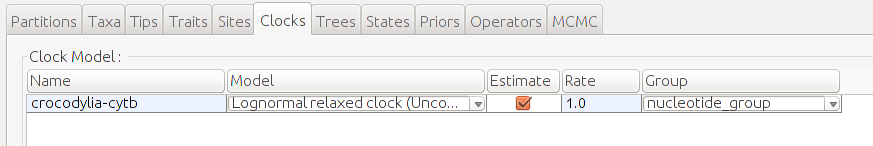
\includegraphics[width=0.8\textwidth]{../screenshots/beauti-clocks-no-geo.jpg}}
        \caption{The clock-model settings.}
        \label{fig:beautiClocks}
    \end{figure}
}

\step{Select the tree prior.}{
    Next, let's move to the \menutab{Trees} tab to specify the prior and
    starting conditions for our tree.
    Select the \fieldvalue{Speciation: Birth-Death Process} option from the
    drop-down for the \field{Tree Prior} option.
    Select \fieldvalue{Random starting tree} in the lower window
    (Figure~\ref{fig:beautiTrees}).

    \begin{figure}[htbp]
        \centering
        \fbox{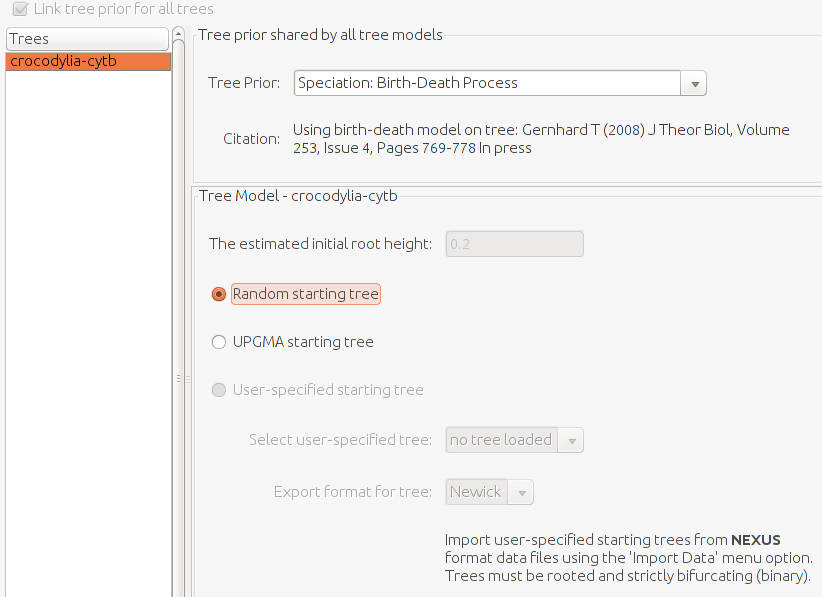
\includegraphics[width=0.8\textwidth]{../screenshots/beauti-trees.jpg}}
        \caption{The tree-prior settings.}
        \label{fig:beautiTrees}
    \end{figure}

    BEAUTi offers a number of tree prior options. Those labeled
    \fieldvalue{Speciation} are based on stochastic branching processes that
    assume the tips of the phylogeny are species. The \fieldvalue{Coalescent}
    tree priors are based on stochastic processes of lineage coalescence that
    assume the tips of the tree are gene copies within a population.
}

% \step{Set the \field{States} options.}{
%     Move to the \menutab{States} tab.
%     With the \fieldvalue{crocodylia-cytb} \field{Partition} selected in the
%     left column, leave all of the settings unchecked and the \field{Error
%     Model} \fieldvalue{Off} (Figure~\ref{fig:beautiCytbStates}).
%     Next, select the \fieldvalue{geography} \field{Partition} in the left column,
%     check the \field{Reconstruct states at all ancestors} box, and leave all other
%     options unchecked (Figure~\ref{fig:beautiGeoStates}).

%     \begin{figure}[htbp]
%         \centering
%         \fbox{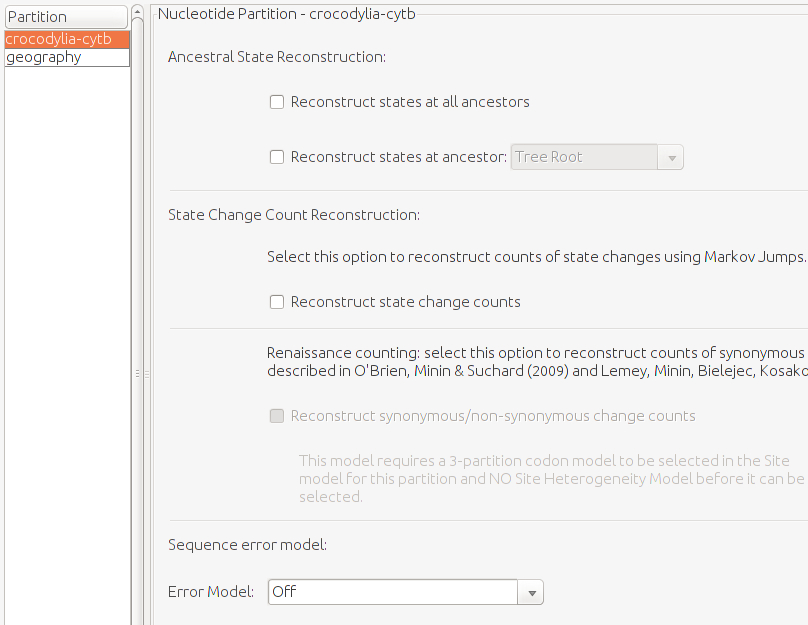
\includegraphics[width=0.7\textwidth]{../screenshots/beauti-cytb-states.jpg}}
%         \caption{The \menutab{States} settings for cytb.}
%         \label{fig:beautiCytbStates}
%     \end{figure}
%     \begin{figure}[htbp]
%         \centering
%         \fbox{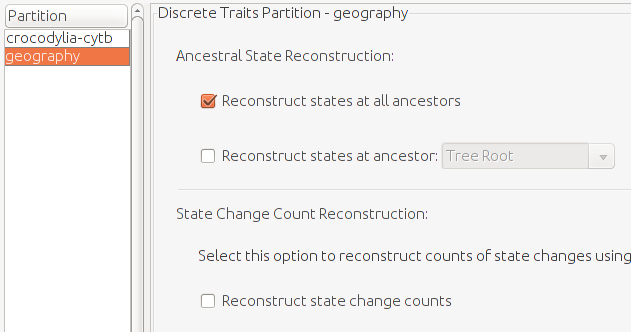
\includegraphics[width=0.5\textwidth]{../screenshots/beauti-geo-states.jpg}}
%         \caption{The \menutab{States} settings for geography.}
%         \label{fig:beautiGeoStates}
%     \end{figure}
% }

\step{Select priors for parameters.}{
    Move to the \menutab{Priors} tab.
    Here we see that all of the model parameters and statistics that we
    specified under the other tabs are listed.
    Now, we can specify prior probability distributions on the
    substitution-model parameters, relaxed-clock parameters, tree-prior
    parameters, and the time (age) of the most recent common ancestor (TMRCA)
    of the taxon sets we specified earlier.

    Let's start by selecting priors for the \fieldvalue{CP1.mu},
    \fieldvalue{CP2.mu}, and \fieldvalue{CP3.mu} parameters. These are
    relative-rate parameters that allow sites at the three codon positions to
    evolve at different rates. Based on our knowledge of the redundancy of the
    genetic code, we expect the sites at third-codon position to evolve more
    rapidly than the first and second codon sites \emph{a priori}.
    So we will specify our priors accordingly.

    Click on the \field{Prior} column for the \fieldvalue{CP1.mu} parameter.
    In the window that pops up, select an \fieldvalue{Exponential} \field{Prior
    Distribution}, and specify a \field{Mean} of \fieldvalue{0.5}.
    Do the same for \fieldvalue{CP2.mu}.
    For \fieldvalue{CP3.mu}, also select an \fieldvalue{Exponential}
    \field{Prior}, but set the \field{Mean} to \fieldvalue{5.0}
    (Figure~\ref{fig:beautiPriorsCPmu}).

    \begin{figure}[htbp]
        \centering
        \begin{subfigure}[b]{0.3\textwidth}
            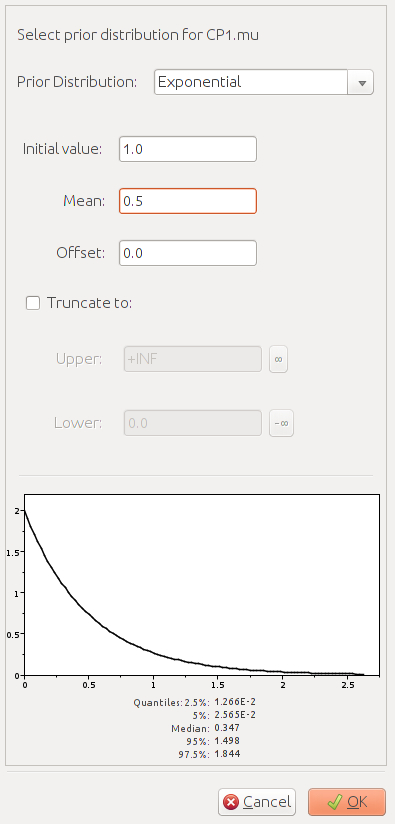
\includegraphics[width=\textwidth]{../screenshots/beauti-prior-cp1mu.jpg}
            \caption{CP1.mu.}
            \label{fig:beautiPriorsCP1mu}
        \end{subfigure}
        \begin{subfigure}[b]{0.3\textwidth}
            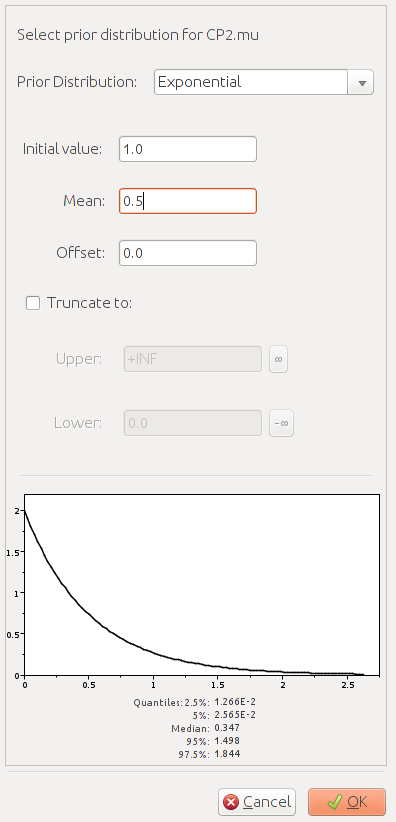
\includegraphics[width=\textwidth]{../screenshots/beauti-prior-cp2mu.jpg}
            \caption{CP2.mu.}
            \label{fig:beautiPriorsCP2mu}
        \end{subfigure}
        \begin{subfigure}[b]{0.3\textwidth}
            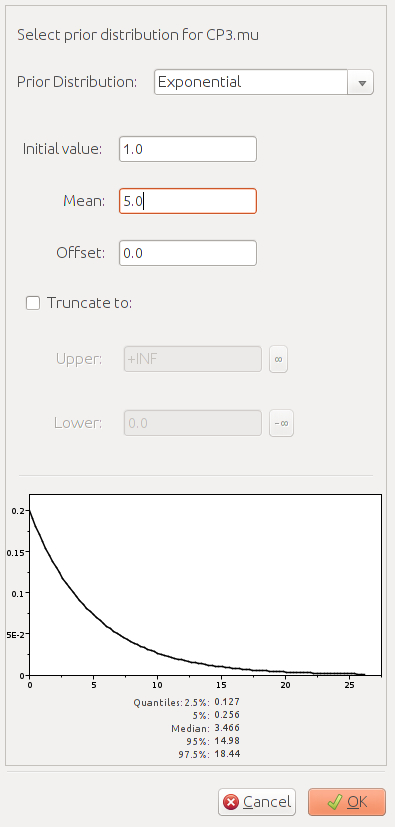
\includegraphics[width=\textwidth]{../screenshots/beauti-prior-cp3mu.jpg}
            \caption{CP2.mu.}
            \label{fig:beautiPriorsCP3mu}
        \end{subfigure}
        \caption{Priors for relative-rate parameters.}
        \label{fig:beautiPriorsCPmu}
    \end{figure}

    \begin{figure}[htbp]
        \centering
        \begin{subfigure}[b]{0.3\textwidth}
            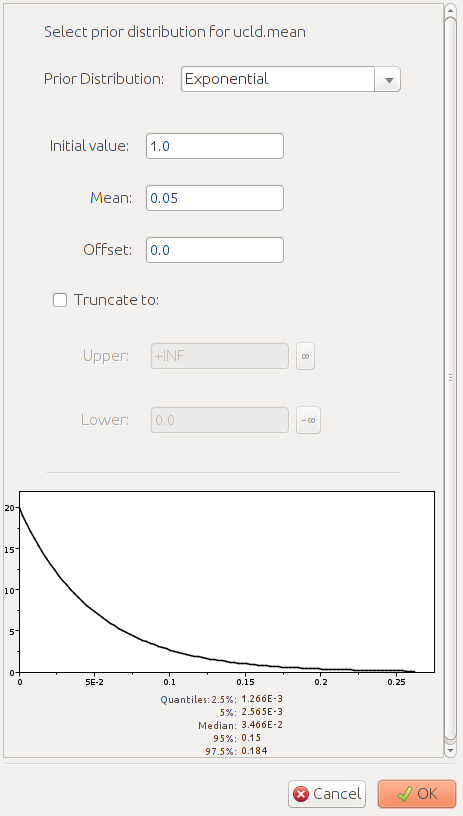
\includegraphics[width=\textwidth]{../screenshots/beauti-prior-ucldmean-no-geo.jpg}
            % \caption{crocodylia-cytb.ucld.mean.}
            \caption{ucld.mean.}
            \label{fig:beautiPriorsUcldMean}
        \end{subfigure}
        % \begin{subfigure}[b]{0.29\textwidth}
        %     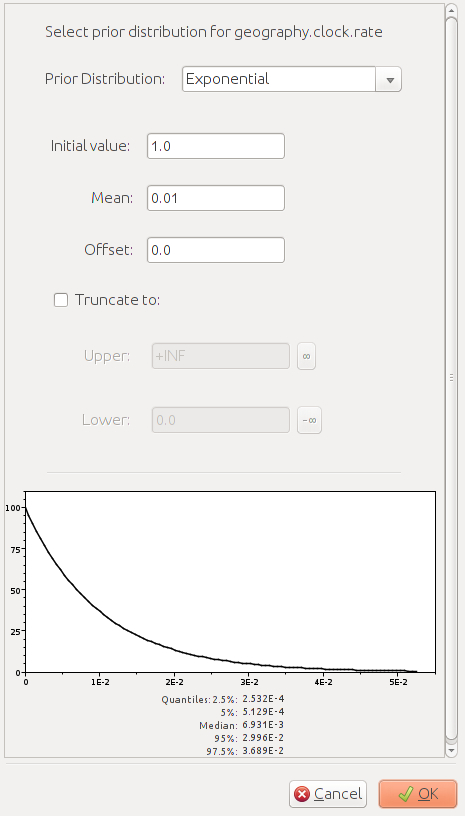
\includegraphics[width=\textwidth]{../screenshots/beauti-prior-clockrate.jpg}
        %     \caption{geography.clock.rate.}
        %     \label{fig:beautiPriorsClockRate}
        % \end{subfigure}
        \begin{subfigure}[b]{0.325\textwidth}
            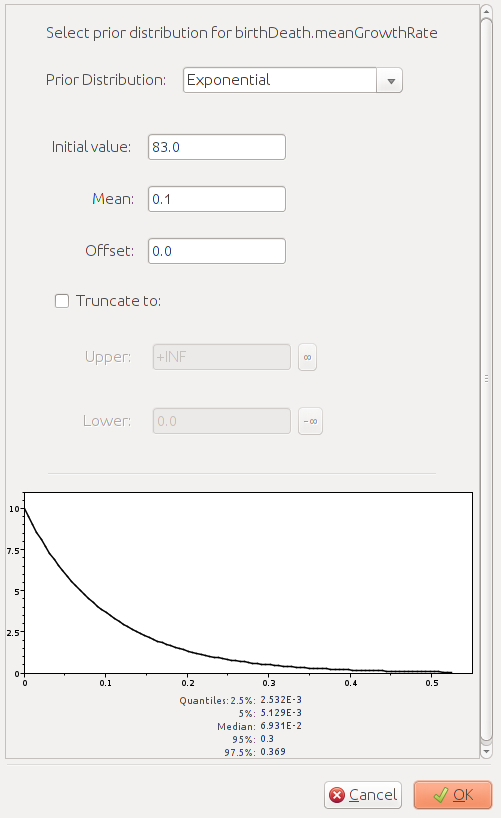
\includegraphics[width=\textwidth]{../screenshots/beauti-prior-birthrate.jpg}
            \caption{birthDeath.meanGrowthRate.}
            \label{fig:beautiPriorsBirthRate}
        \end{subfigure}
        \caption{Priors for clock rates and diversification rate.}
        \label{fig:beautiPriorsClocks}
    \end{figure}
    
    Next, click on the \field{Prior} column for the
    % \fieldvalue{crocodylia-cytb.ucld.mean} parameter.
    \fieldvalue{ucld.mean} parameter.
    This parameter controls the mean of the log-normal distribution from which
    the rates of each branch of the tree are drawn.
    Because we will be using fossils to calibrate the overall rate of substitution,
    we will use a very diffuse prior for this parameter.
    Select \fieldvalue{Exponential} for the \field{Prior}
    and specify \fieldvalue{0.05} for the \field{Mean}
    (Figure~\ref{fig:beautiPriorsUcldMean}).
    Because we will be specifying node-age priors in units of millions of
    % years, the mean of 0.05 for prior on \fieldvalue{crocodylia-cytb.ucld.mean}
    years, the mean of 0.05 for prior on \fieldvalue{ucld.mean}
    translates to a mean rate of 5\% per million years.

    % Specify an \fieldvalue{Exponential} prior for the
    % \fieldvalue{geography.clock.rate}, but with a \field{Mean} of
    % \fieldvalue{0.01} (Figure~\ref{fig:beautiPriorsClockRate}).

    The default prior for the \fieldvalue{birthDeath.meanGrowthRate}
    is \fieldvalue{Uniform} from \fieldvalue{0} to \fieldvalue{10000}.
    This is a very broad prior.
    Based on our knowledge of the crocodylian fossil record, we can get
    a rough idea of our prior expectations for this parameter.
    Given the age of the oldest crocodylian fossil is 71.3 million
    years, we know the height of our tree is at least that.
    Given that, we can calculate a pure-birth (Yule process) rate that has an
    expected tree height of 71.3 million years.
    I have included a Python script \localfile{yule.py} in the tutorial
    download that performs such calculations.
    This program is hosted via \href{http://git-scm.com/}{git} on
    \href{https://github.com/}{GitHub} at
    \href{https://github.com/joaks1/pyule.git}{\url{https://github.com/joaks1/pyule.git}};
    license information and documentation are available on the GitHub site.

    You do not have to do this now, but if you open a \program{Terminal}
    window and invoke the script as follows:

    \hspace{1cm}\cmd{python yule.py height 71.3 24}

    you get the following output:

    \cmd{ntips = 24}\\
    \cmd{rate = 0.0389334947792}\\
    \cmd{height = 71.3}\\
    \cmd{length = 590.750974976}

    From these results, we see that the largest we expect a pure-birth rate to
    be is around 0.04.
    This allows us to specify a much better prior than the default.
    Specify an \fieldvalue{Exponential} prior for the
    \fieldvalue{birthDeath.meanGrowthRate}, but with a \field{Mean} of
    \fieldvalue{0.1} (Figure~\ref{fig:beautiPriorsBirthRate}).


    You will also specify an \fieldvalue{Exponential} prior for the
    \fieldvalue{ucld.stdev} parameter.
    {\color{red}We will assign you a value to specify for the \field{Mean} of
    this distribution.}
    At the end of the lab we will compare are our findings to see how sensitive
    the analysis is to this prior.
}

\step{Select priors for node ages!}{
    Next, we need to specify our node-age priors based on fossil information.

    For \fieldvalue{tmrca(Alligatoridae)} select \fieldvalue{Gamma} for the
    \field{Prior Distribution}, and specify \fieldvalue{2} for both the
    \field{Shape} and \field{Scale} and \fieldvalue{64} for the
    \field{Offset}
    (Figure~\ref{fig:beautiPriorsAlligatoridae}).

    For \fieldvalue{tmrca(Crocodylus)} select \fieldvalue{Exponential} for the
    \field{Prior Distribution}, and specify \fieldvalue{10} for the mean
    and \fieldvalue{12} for the \field{Offset}
    (Figure~\ref{fig:beautiPriorsCrocodylus}).

    For \fieldvalue{tmrca(Caiman)} select \fieldvalue{Exponential} for the
    \field{Prior Distribution}, and specify \fieldvalue{4} for the mean
    and \fieldvalue{9} for the \field{Offset}
    (Figure~\ref{fig:beautiPriorsCaiman}).

    For \fieldvalue{treeModel.rootHeight} select \fieldvalue{Gamma} for the
    \field{Prior Distribution}, and specify \fieldvalue{78} for the
    \field{Initial value}, \fieldvalue{1.5} for the \field{Shape},
    \fieldvalue{6.0} for the \field{Scale}, and \fieldvalue{71.3} for the
    \field{Offset}. Also, make sure \field{Truncate to} is unchecked
    (Figure~\ref{fig:beautiPriorsRoot}).

    \begin{figure}[htbp]
        \centering
        \begin{subfigure}[b]{0.33\textwidth}
            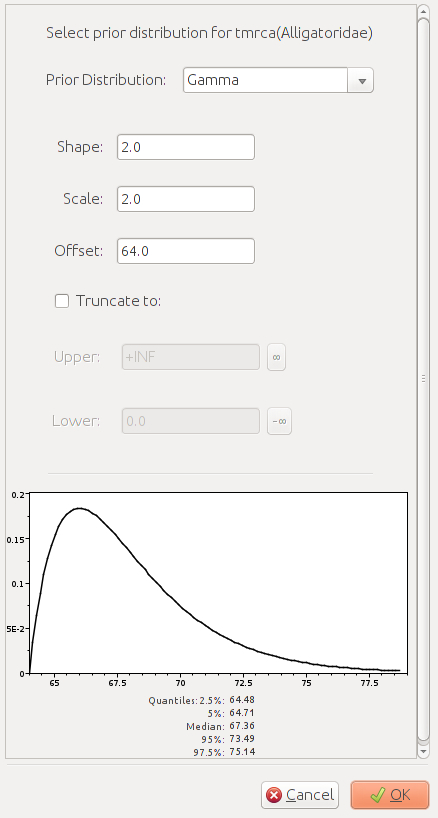
\includegraphics[width=\textwidth]{../screenshots/beauti-prior-alligatoridae.jpg}
            \caption{tmrca(Alligatoridae).}
            \label{fig:beautiPriorsAlligatoridae}
        \end{subfigure}
        \begin{subfigure}[b]{0.35\textwidth}
            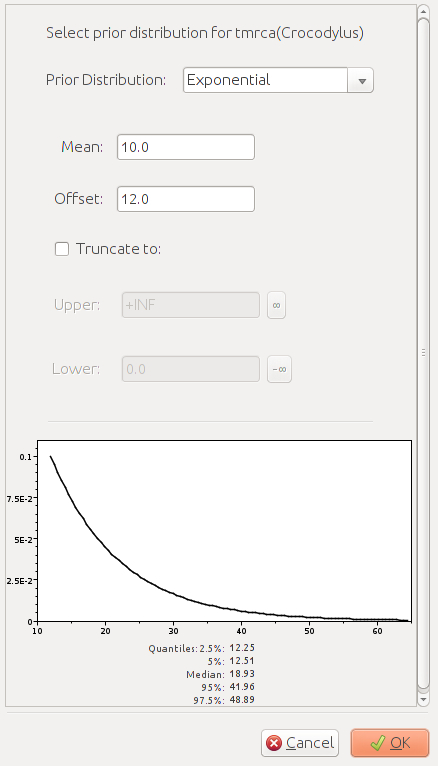
\includegraphics[width=\textwidth]{../screenshots/beauti-prior-crocodylus.jpg}
            \caption{tmrca(Crocodylus).}
            \label{fig:beautiPriorsCrocodylus}
        \end{subfigure}
        \begin{subfigure}[b]{0.35\textwidth}
            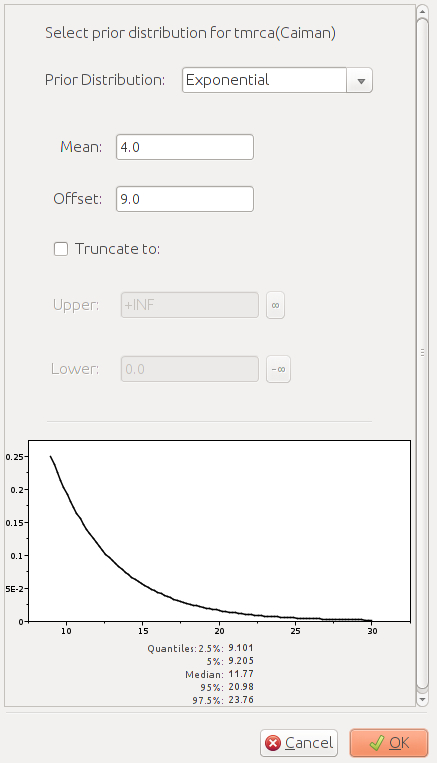
\includegraphics[width=\textwidth]{../screenshots/beauti-prior-caiman.jpg}
            \caption{tmrca(Caiman).}
            \label{fig:beautiPriorsCaiman}
        \end{subfigure}
        \begin{subfigure}[b]{0.315\textwidth}
            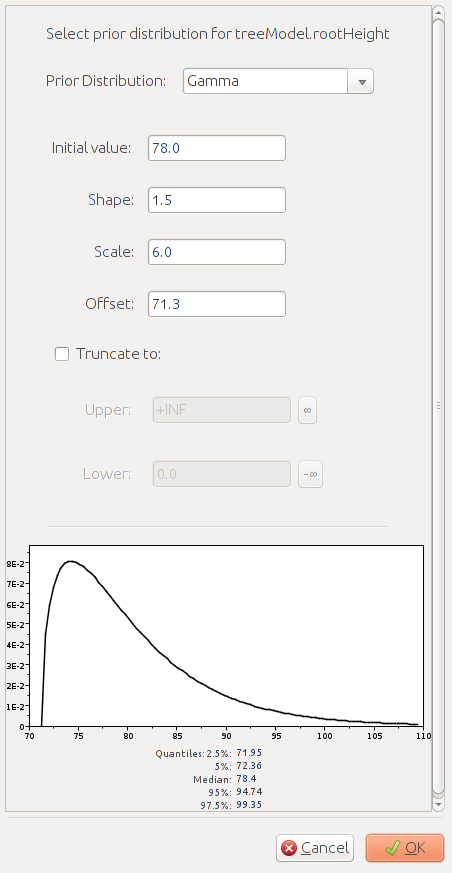
\includegraphics[width=\textwidth]{../screenshots/beauti-prior-root.jpg}
            \caption{treeModel.rootHeight.}
            \label{fig:beautiPriorsRoot}
        \end{subfigure}
        \caption{Priors for clock rates and diversification rate.}
        \label{fig:beautiPriorsClocks}
    \end{figure}

    After setting all the above priors, your \menutab{Priors} tab window should
    look like Figure~\ref{fig:beautiPriors}.

    \begin{figure}[htbp]
        \centering
        \fbox{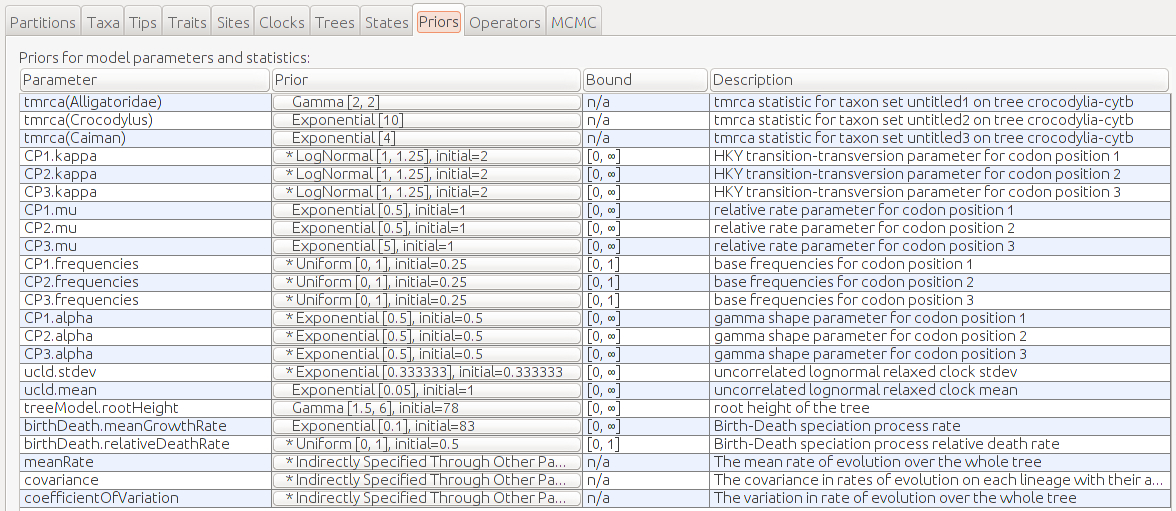
\includegraphics[width=1.0\textwidth]{../screenshots/beauti-priors.jpg}}
        \caption{The prior settings.}
        \label{fig:beautiPriors}
    \end{figure}
}

\step{Specify MCMC settings and generate \beast XML files.}{
    Next, move to the \menutab{MCMC} tab.
    Change the following settings:
    \begin{compactdesc}
        \centering
        \item[\field{Length of chain:}] \fieldvalue{1000000} (1 million)
        \item[\field{Echo state to screen every:}] \fieldvalue{1000}
        \item[\field{Log parameters every:}] \fieldvalue{1000}
    \end{compactdesc}
    Leave the remaining options at their default values
    (Figure~\ref{fig:beautiMCMC}).

    \begin{figure}[htbp]
        \centering
        \fbox{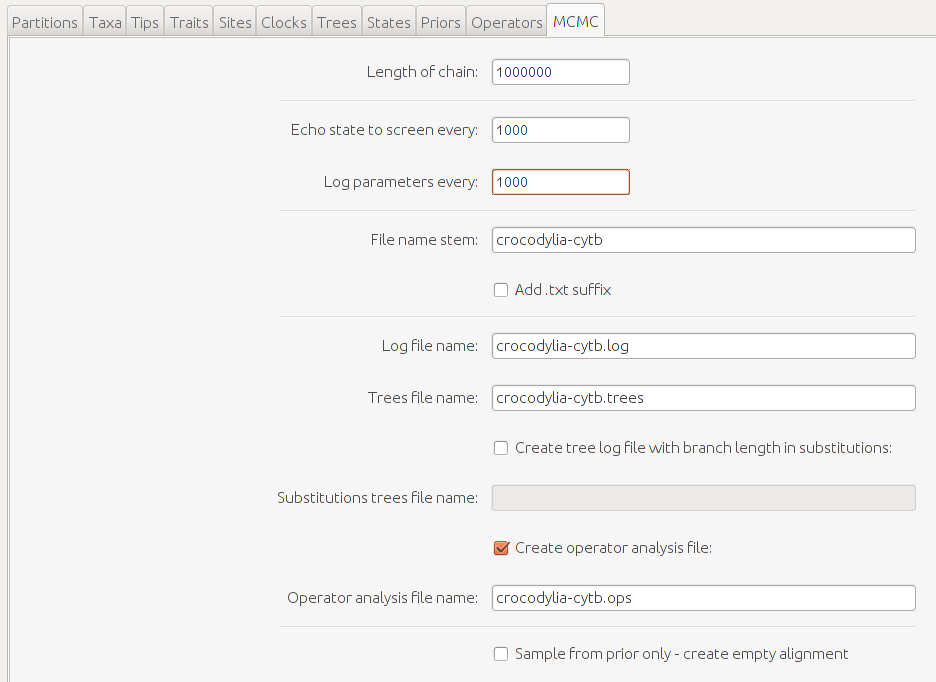
\includegraphics[width=1.0\textwidth]{../screenshots/beauti-mcmc.jpg}}
        \caption{The MCMC settings.}
        \label{fig:beautiMCMC}
    \end{figure}

    Next, click the \field{Generate BEAST File\ldots} in the bottom-right
    corner of the window.
    A subwindow will pop up warning you that some of the priors are still at
    their default values.
    You can ignore this and click \field{Continue}.
    Another subwindow will appear for specifying the name and location for
    saving the XML file. You can leave the name the same and save the file to
    the \localfile{div-time-tutorial} folder on your desktop.

    Due to time constraints, in this lab we are running a single, short
    MCMC chain to sample from the joint posterior distribution of the model we
    just finished specifying.
    As a result, the posterior estimates will have a large amount of
    MCMC sampling error.
    For a dataset of this size, and a model with this many parameters, we need
    to run a longer chain in BEAST to get a more robust sample from the
    posterior.
    We will not do this today, but in general, you should always run multiple,
    independent MCMC analyses in order to increase the posterior sample size,
    and to help assess whether the chains converged to the same stationary
    distribution.
    Also, you should always run an MCMC analysis that samples from the joint
    prior distribution (i.e., an analysis that ignores the data).  This allows
    you to evaluate the interaction of all the priors you have specified for
    the various parameters, and also gives you an idea of how much the data are
    influencing certain parameter estimates.
    We will not do this today, but you do this by checking the \field{Sample
    from prior only-create empty alignment} box and creating another XML file
    (make sure you change the name!).

    Later, when your analysis is running, we will look at results from multiple,
    longer chains and from a chain that sampled only from the prior.
}

\intermediate{\subsection{Running the XML file with \beast}}

\step{Run the XML file in \beast.}{
    Launch the \beast program. If you are using Mac OSX or Windows, you should
    be able to do this by double clicking on the application. 
    After the \beast window appears, click the \field{Choose File\ldots} button,
    and select the XML file you just created (Figure~\ref{fig:beast}).
    Click \field{Run}. The analysis should take about 20 minutes.

    \begin{figure}[htbp]
        \centering
        \fbox{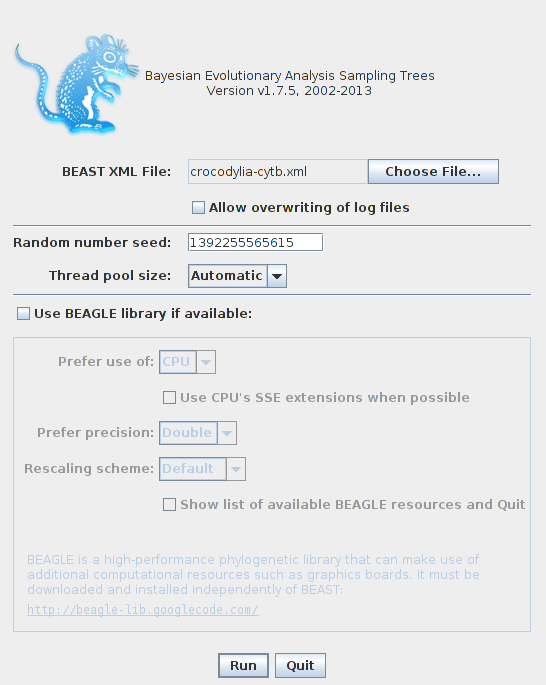
\includegraphics[width=0.5\textwidth]{../screenshots/beast.jpg}}
        \caption{The \beast GUI window.}
        \label{fig:beast}
    \end{figure}
}

\intermediate{\subsection{Inspecting previous results with \program{Tracer}}}

\intermediate{
    In the \localfile{div-time-tutorial} folder, there is a subfolder called
    \localfile{output} containing \localfile{.log} and \localfile{.trees} files
    from analyses I ran previously.
}

\step{Inspect previous results with \program{Tracer}.}{
    Launch the \program{Tracer} program.
    Load the \localfile{crocodylia-cytb-run1.log} and
    \localfile{crocodylia-cytb-run2.log} in the \localfile{output} directory
    into
    \program{Tracer} using \subItem{File}{Import Trace File\ldots} or the
    \plusbutton button.

    Use Tracer to inspect the behavior of the two MCMC chains.

    \question{Does it look like the chains reached stationarity?}

    \question{Does it look like both chains converged to the same stationarity
    distribution?}

    \question{What do we call this stationary distribution?}

    Now, load the \localfile{crocodylia-cytb-prior.log} file into
    \program{Tracer}.
    This log file is from the analysis that sampled only from the prior
    distribution.
    Use \program{Tracer} to compare the prior and posterior samples.

    \question{Are any of the parameter estimates similar between the prior and
    posterior? Which ones?}
}

\intermediate{\subsection{Summarizing the trees with \program{LogCombiner} and \program{TreeAnnotator}}}

\intermediate{
Once you have reviewed the log files from the independent runs in Tracer and determined that they have 
reached stationarity, you can combine the sampled trees into a single tree file.
}

\step{Combine tree files using \program{LogCombiner}.}{
	Launch the \program{LogCombiner} program.
	Change the \field{File type:} to \field{Tree Files}.
	Load the \localfile{crocodylia-cytb-run1.trees} and \localfile{crocodylia-cytb-run2.trees} file in the \localfile{output} directory into
	\program{LogCombiner} using the \plusbutton button.
	Select the \field{Choose File\ldots} button and specify the \localfile{output}
	directory and a file name, \localfile{crocodylia-cytb-runs1and2.trees}.
    Specify an appropriate burn-in value based on what you saw in \program{Tracer}.
	Click \field{Run}
}

\intermediate{Now you have a single tree file with all the trees from the two independent runs called \localfile{crocodylia-cytb-runs1and2.trees}.
TreeAnnotator will summarize the trees and identify the topology with the best posterior support, and summarize the age estimates for each node in the tree.
}

\step{Summarize the trees using \program{TreeAnnotator}.}{
	Launch the \program{TreeAnnotator} program.
    Specify the burnin value as \fieldvalue{0} (we removed the burn-in with \program{LogCombiner}).
	For the \field{Target tree type} field, choose \fieldvalue{Maximum clade credibility tree}.
    For the \field{Node heights} field, choose \fieldvalue{Median heights}.
	Select the \field{Input Tree File} button and select the file \localfile{crocodylia-cytb-runs1and2.trees}.
	Select the \field{Output File} button and specify the \localfile{output} directory and a 
	file name, \localfile{crocodylia-MCC.tre}.
	Click \field{Run}
}

\intermediate{\subsection{Visualizing the tree in \program{FigTree}}}

\step{Look at the summary tree in \program{FigTree}.}{
    Launch the \program{FigTree} program, and load the \localfile{crocodylia-MCC.tre} file
    you just created with \program{TreeAnnotator}.
    Check the \field{Scale Axis} option in the left column, and check the
    \subItem{Scale Axis}{Reverse axis} box.
    Check the \field{Node Bars} option and select
    \fieldvalue{height\_95\%\_HPD} for the \subItem{Node bars}{Display} field.

    \question{What is the age of the most recent common ancestor of all
    \emph{Crocodylus} species?}

    \question{What is the age of the stem node for \emph{Crocodylus}?}
}

\intermediate{\subsection{Inspecting your results with \program{Tracer}}}

\step{Inspect the results of your short analysis with \program{Tracer}.}{

    If your analysis has finished, launch the \program{Tracer} program and load
    the log file created by \program{BEAST}.

    \question{What was the mean you specified for the prior on
    \fieldvalue{ucld.stdev}?}

    \question{What is your estimate of the mean and 95\% HPD interval for the
        age of the stem node for \emph{Crocodylus} (hint: the
        \fieldvalue{tmrca(Crocodylus)} statistic)?}

    \question{Compare your estimate with your classmates that used a different
    prior on \fieldvalue{ucld.stdev}. Are the results sensitive to this prior?
    Is there a trend?}
}
